\documentclass{beamer}
%\usepackage[latin1]{inputenc}
\usepackage{amsmath}
\usepackage{amssymb}
\usepackage{verbatim}
%\usepackage{cite}
\usepackage{booktabs}
\usepackage{multirow}
\usepackage{fancyvrb}
\usepackage{color}
\usepackage[vlined,ruled,commentsnumbered]{algorithm2e}
\usepackage{tikz}

\DeclareMathOperator{\probability}{Pr}
\DeclareMathOperator*{\argmax}{arg\,max}
\DeclareMathOperator*{\argmin}{arg\,min}


\usetheme{Warsaw}
%\usetheme{Copenhagen}

\title{System Modeling, part 2}
%\subtitle{A Library for Ensemble Learning Using Support Vector Machines}
\author{Marc~Claesen}
%\institute{ESAT-STADIUS, KU~Leuven \\ iMinds Medical IT Department}

\definecolor{blueish}{rgb}{0.3,0.3,0.7}

\AtBeginSection[]
{
\begin{frame}<beamer>
\frametitle{Outline}
\tableofcontents[currentsection]
\end{frame}
}

\AtBeginSubsection[]
{
\begin{frame}<beamer>
\frametitle{Outline}
\tableofcontents[currentsubsection]
\end{frame}
}

%\AtBeginSubsubsection[]
%{
%\begin{frame}<beamer>
%\frametitle{Outline}
%\tableofcontents[currentsubsection]
%\end{frame}
%}

%% let pdflatex show eps figs
\newif\ifpdf
\ifx\pdfoutput\undefined
\pdffalse
\else
\pdfoutput=1
\pdftrue
\fi
\ifpdf
\usepackage{graphicx}
\usepackage{epstopdf}
%nessim
\epstopdfsetup{suffix=}
\DeclareGraphicsRule{.eps}{pdf}{.pdf}{`epstopdf #1}
\pdfcompresslevel=9
\else
\usepackage{graphicx}
\fi

\begin{document}
%\nocite{*}

\begin{frame}
\titlepage
\end{frame}

\begin{frame}
\tableofcontents
\end{frame}

\section{Nonlinear systems \& linearization}
\begin{frame}
\frametitle{Nonlinear systems}
In this course we focus on the linear state-space representation:
\begin{align*}
\left\{ \begin{matrix} 
\dot{x}(t) = A x(t) + B u(t), \\ 
y(t) = C x(t) + D u(t).
\end{matrix}\right.\quad\quad
\left\{ \begin{matrix} 
x[k+1] &= A x[k] + B u[k], \\ 
y[k] &= C x[k] + D u[k].
\end{matrix}\right.
\end{align*}
\pause
\ \newline
Most real life systems involve nonlinearity:
\begin{align*}
\left\{ \begin{matrix} 
\dot{x}(t) = f\big(x(t), u(t)\big), \\ 
y(t) = g\big(x(t), u(t)\big),
\end{matrix}\right.
\end{align*}
\pause
where $f$ and/or $g$ contain some nonlinearity, such as:
\pause
\begin{itemize}
\item \emph{powers}: e.g. $\dot{x}(t) = A x(t) + B u(t) {\color{blue}+ \gamma u(t)^2}$,
\pause
\item \emph{interactions}: e.g. $\dot{x}(t) = A x(t) + B u(t) {\color{blue}+ \gamma x(t) u(t)}$,
\pause
\item \emph{clipping}: e.g. ${\color{blue}\alpha \leq }x(t){\color{blue}\leq \beta}$.
\end{itemize}
\end{frame}

\begin{frame}
\frametitle{Linearization around equilibrium point}
\pause
Nonlinear systems have (several) equilibrium points $x_e$, $u_e$, $y_e$:
\begin{align*}
\left\{ \begin{matrix}
\dot{x}_e = f\big(x_e, u_e\big)=0, \hfill \\
y_e = g\big(x_e, u_e\big). \hfill
\end{matrix}\right.
\end{align*}
\pause
Linearizing in the region of $(x_e, u_e, y_e)$:
\begin{align*}
x = x_e + \Delta x, \quad u = u_e + \Delta u, \quad y = y_e + \Delta y,
\end{align*}
\pause
with $\Delta x$, $\Delta u$ and $\Delta y$ \emph{sufficiently} small.\\
\ \newline
\pause
Linearizing is done via first order Taylor expansions:
\begin{align*}
\left\{ \begin{matrix}
\frac{dx}{dt} = \frac{d\Delta x}{dt} = f(x,u) = f(x_e+\Delta x, u_e + \Delta u), \\
y_e + \Delta y = g(x, u) = g(x_e + \Delta x, u_e + \Delta u).
\end{matrix}\right.
\end{align*}
\end{frame}

\begin{frame}
\frametitle{Example: decalcification plant}
Used to reduce concentration of calcium hydroxide in water:
\begin{itemize}
\item chemical reaction: $Ca(OH)_2 + CO_2 \rightarrow CaCO_3 + H_2O$
\item reaction speed: $r = c[Ca(OH)_2][CO_2]$
\item rate of change of concentration:
\begin{align*}
\frac{d[Ca(OH)_2]}{dt} = \frac{k}{V} - \frac{r}{V}, \\
\frac{d[CO_2]}{dt} = \frac{u}{V} - \frac{r}{V}, 
\end{align*}
with inflow rates $k$ and $u$ in mol/s and tank volume $V$ in L.
\item input $u$: inflow of $CO_2$, output: $[Ca(OH)_2]$
\end{itemize}
\end{frame}

\begin{frame}
\frametitle{Nonlinear model and equilibrium point}
{\color{red}Nonlinear} model for the given reactor:
\pause
\begin{align*}
\frac{d[Ca(OH)_2]}{dt} &= \frac{k}{V} - \frac{c}{V}{\color{red}[Ca(OH)_2][CO_2]}, \\
\frac{d[CO_2]}{dt} &= \frac{u}{V} - \frac{c}{V}{\color{red}[Ca(OH)_2][CO_2]}, \\
y &= [Ca(OH)_2],
\end{align*}
with two state variables: ${\color{blue}x_1=[Ca(OH)_2]}$ and ${\color{blue}x_2=[CO_2]}$.\\
\ \newline
\pause
The equilibrium point ${\color{blue}(k_{eq}, u_{eq}, x_{1,eq}, x_{2,eq}, y_{eq})}$ of this system is:
\pause
\begin{align*}
\frac{{\color{blue}k_{eq}}}{V} - \frac{c}{V}{\color{blue}[Ca(OH)_2]_{eq}[CO_2]_{eq}} = 0, \\
\frac{{\color{blue}u_{eq}}}{V} - \frac{c}{V}{\color{blue}[Ca(OH)_2]_{eq}[CO_2]_{eq}} = 0. \\
\end{align*}
\end{frame}

\begin{frame}
\frametitle{Linearization of the decalcification plant}
For small deviations near the equilibrium:
\begin{align*}
\frac{d{\color{blue}\Delta x_1}}{dt} &= -\frac{c}{V} [CO_2]_{eq} {\color{blue}\Delta x_1} - \frac{c}{V} [Ca(OH)_2]_{eq} {\color{blue}\Delta x_2}, \\
\frac{d{\color{blue}\Delta x_2}}{dt} &= -\frac{c}{V} [CO_2]_{eq} {\color{blue}\Delta x_1} - \frac{c}{V} [Ca(OH)_2]_{eq} {\color{blue}\Delta x_2} + \frac{{\color{blue}\Delta u}}{V}, \\
{\color{blue}\Delta y} &= {\color{blue}\Delta x_1}.
\end{align*}
\pause
The resulting linear state-space model is $\begin{aligned}\left\{ \begin{matrix} \dot{x}(t) = {\color{green!70!black}A}x(t) + {\color{red}B}u(t) \\ y(t) = Cx(t) + Du(t) \end{matrix}\right.\end{aligned}$:
\pause
\begin{align*}
\begin{bmatrix}
\frac{d[Ca(OH)_2]}{dt} \\
\frac{d[CO_2]}{dt}
\end{bmatrix} &= 
{\color{green!70!black}
-\begin{bmatrix}
\frac{c}{V}[CO_2]_{eq} & \frac{c}{V}[Ca(OH)_2]_{eq} \\
\frac{c}{V}[CO_2]_{eq} & \frac{c}{V}[Ca(OH)_2]_{eq} \\
\end{bmatrix}}
\begin{bmatrix}
[Ca(OH)_2] \\
[CO_2]
\end{bmatrix} +
{\color{red}
\begin{bmatrix}
0 \\
\frac{1}{V} \\
\end{bmatrix}} u(t) \\
y(t) &= [Ca(OH)_2]
\end{align*}
\end{frame}


\section{System identification (cont)}
\begin{frame}
\frametitle{Main classes of identification methods}
\textbf{White box modeling}: based on first principles. \\
\pause
$\rightarrow$ known equations (structure) $\&$ parameters (coefficients). \\
\ \newline
\pause
\textbf{Grey box identification}: first principles $\&$ experimentation. \\
\pause
$\rightarrow$ known equations, unknown/uncertain parameters. \\
\ \newline
\pause
\textbf{Black box identification}: based on experimentation. \\
\pause
$\rightarrow$ unknown equations $\&$ unknown parameters. \\
\ \newline
\pause
Most popular approaches are forms of black box identification.
\end{frame}

\subsection{Grey box identification}
\begin{frame}
\frametitle{Grey box identification: conceptual}
\pause
Grey box identification starts from a known model structure but with unknown/uncertain parameters $\leftrightarrow$ \textbf{parametric statistics}. \\
\pause
\ \newline
We assume linear, continuous time state space representation:
\begin{align*}
\left\{ \begin{matrix} 
\dot{x}(t) = {\color{blue}A}x(t) + {\color{blue}B}u(t), \\ 
y(t) = {\color{blue}C}x(t) + {\color{blue}D}u(t).
\end{matrix}\right.
\end{align*}
\pause
\textbf{Given}: states, inputs, outputs and guesstimates of $\tilde{A}$, $\tilde{B}$, $\tilde{C}$ $\&$ $\tilde{D}$.
\pause
\textbf{Task}: estimate $\hat{A}$, $\hat{B}$, $\hat{C}$ and $\hat{D}$ adequately via experiments.\\
\ \newline
\pause
``\emph{All models are wrong, but some are useful.}'' \hfill - George E. P. Box
\end{frame}

\begin{frame}
\frametitle{Linear regression}
Consider input matrix $\mathbf{X}$, output vector $\mathbf{y}$ and residuals $\epsilon$:
\begin{align*}
\mathbf{X}\theta &= \mathbf{y} + \epsilon.
\end{align*}
The parameter vector $\theta$ must be estimated, given the observations.\\
\pause
\ \newline
A common estimation approach is ordinary least squares (OLS):
\begin{align*}
(\mathbf{X}^T\mathbf{X})\hat{\theta}_{OLS} &= \mathbf{X}^T\mathbf{y}, \\
\hat{\theta}_{OLS} &= (\mathbf{X}^T\mathbf{X})^{-1} \mathbf{X}^T\mathbf{y}.
\end{align*}
\pause
The OLS estimate minimizes the sum-of-squares of errors, i.e.:
\begin{equation*}
\hat{\theta}_{OLS} = \argmin_{\theta} \sum_{i=1}^N \big(y(i) - \sum_{j=1}^d X(i,j)\theta(j)\big)^2
\end{equation*}
\end{frame}

\begin{frame}
\frametitle{Linear regression with ordinary least squares}
\begin{figure}[!h]
  \centering
  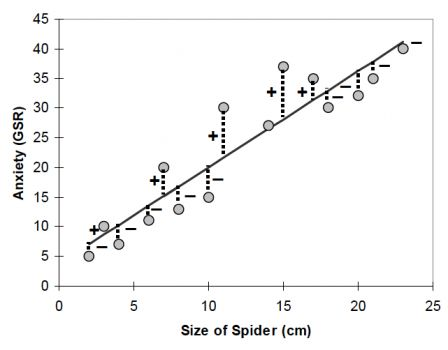
\includegraphics[width=0.8\textwidth]{linear-regression.jpg}
\end{figure}
\tiny{Image taken from \url{http://freakonometrics.hypotheses.org/2348}}.
\end{frame}


\begin{frame}
\frametitle{Maximum likelihood estimation}
The maximum likelihood estimate $\hat{\theta}_{ML}$ is the parameter vector that maximizes the likelihood $\mathcal{L}(\cdot)$ of observing the (known) outputs $\mathbf{y}$, given the (known) inputs $\mathbf{X}$:
\begin{equation*}
\hat{\theta}_{ML} = \argmax_{\theta} \mathcal{L}\big(\mathbf{y}, \mathbf{X}\ |\ \theta \big)
\end{equation*}
\pause
For some structures, ML estimate can be obtained in closed form.\\
\ \newline
\pause
\textbf{Example}: least squares estimators are the maximum likelihood estimators if the associated residuals $\epsilon$ are normally distributed.
\end{frame}

\begin{frame}
\frametitle{Maximum a posteriori (MAP) estimation}
Bayesian: maximum likelihood estimation with a \emph{prior} $p(\theta)$. \\
$\rightarrow$ MAP estimation is a regularization of ML estimation \\
\ \newline
\pause
Bayes' theorem: $P(A\ |\ B) = P(B\ |\ A) \cdot P(A)\ /\ P(B)$.\\
\ \newline
\pause
If a prior distribution $p(\cdot)$ is available for $\theta$, then the posterior distribution for $\theta$ becomes:
\begin{equation*}
\theta \mapsto \mathcal{L}(\theta\ |\ \mathbf{y}, \mathbf{X}) = \frac{\mathcal{L}(\mathbf{y}, \mathbf{X}\ |\ \theta)p(\theta)}{\int_\vartheta \mathcal{L}(\mathbf{y}, \mathbf{X}\ |\ \vartheta)p(\vartheta)d\vartheta}.
\end{equation*}
\pause
The MAP estimate is the mode of the posterior distribution of $\theta$:
\begin{equation*}
\hat{\theta}_{MAP} = \argmax_{\theta} \mathcal{L}(\mathbf{y}, \mathbf{X}\ |\ \theta) p(\theta).
\end{equation*}

\end{frame}

\begin{frame}
\frametitle{Errors-in-variables approach}
Additionally accounts for {\color{red}measurement errors in inputs}.\\
$\leftrightarrow$ standard regression only accounts for {\color{blue}errors in \emph{outputs}} \\
\ \newline
\pause
Typically described via \emph{latent variables}:
\begin{align*}
\left\{ \begin{matrix}
x = x^\star {\color{red}+ \eta}, \\
y = y^\star {\color{blue}+ \epsilon}, \\
y^\star = g(x^\star\ |\ \theta),
\end{matrix}\right.
\end{align*}
with $x$, $y$ the observed inputs, outputs and latent variables $x^\star$, $y^\star$.\\
\pause
\textbf{Assumption}: latent variables $x^\star$ and $y^\star$ exist which follow the true functional relationship $g(\cdot)$.\\
\ \newline
\pause
\textbf{Task}: estimate $\theta$.
\end{frame}



\subsection{Black box identification}
\begin{frame}
\frametitle{Black box identification}
Start from unknown equations $\&$ unknown parameters. \\
$\rightarrow$ related to \textbf{machine learning} and \textbf{nonparametric statistics}. \\
\pause
\ \newline
If we assume a linear state space system:
\begin{align*}
\left\{ \begin{matrix} 
\dot{x}(t) = A x(t) + B u(t), \\ 
y(t) = C x(t) + D u(t).
\end{matrix}\right.\quad\quad
\left\{ \begin{matrix} 
x[k+1] &= A x[k] + B u[k], \\ 
y[k] &= C x[k] + D u[k].
\end{matrix}\right.
\end{align*}
\pause
\ \newline
Black box identification deals with:
\pause
\begin{itemize}
\item unknown states, both in number $\&$ physical interpretation \\
\pause
$\rightarrow$ dimensions of $A$, $B$ $\&$ $C$ unknown
\pause
\item unknown parameters (values in $A$, $B$, $C$, $D$)
\end{itemize}
\end{frame}

\begin{frame}
\frametitle{Time series: Santa Fe laser}
\begin{figure}[!h]
  \centering
  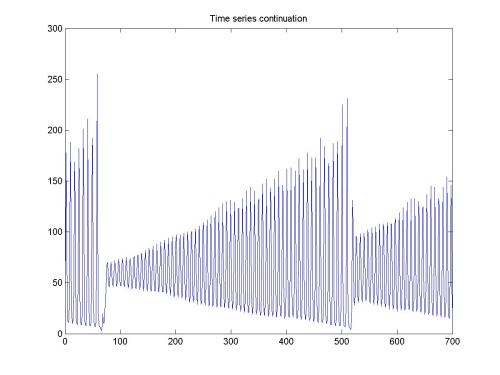
\includegraphics[width=0.8\textwidth]{santafe-full.jpg}
\end{figure}
\end{frame}

\begin{frame}
\frametitle{Modelling the Santa Fe laser}
This laser can be treated as an autonomous discrete time system:
\begin{align*}
\left\{ \begin{matrix} 
x[k+1] = f\big(x[k-N+1], \ldots, x[k]\big), \\
y[k] = x[k]. \hfill
\end{matrix}\right.
\end{align*}
The output depends on the past $N$ states $\&$ no inputs.\\
\pause
$\rightarrow$ how large is $N$? $\rightarrow$ \textbf{unknown structure} \\
\ \newline
\pause
Treat it as a regression problem with $N$ inputs: $y = f\big(X_1,\ldots,X_N\big)$. \\
\pause
$\rightarrow$ lets say linear, i.e. $y = \mathbf{X}\theta$ $\rightarrow$ \textbf{unknown parameters $\theta \in \mathbb{R}^N$}. \\
\pause
$\rightarrow$ for given $N$, we can estimate $\theta$ via grey box methods.\\
\ \newline
\pause
Nonlinear models can be obtained via machine learning methods.
$\rightarrow$ neural networks, support vector machine, random forest, ...
\end{frame}

\begin{frame}
\frametitle{Predictions of a least-squares support vector machine}
\begin{figure}[!h]
  \centering
  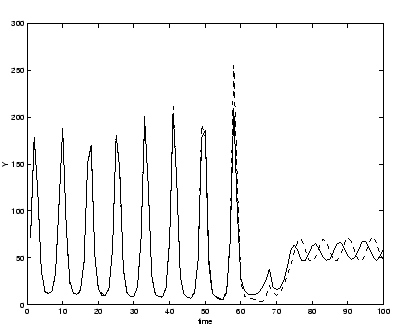
\includegraphics[width=0.8\textwidth]{santafe-prediction.png}
\end{figure}
\end{frame}


\begin{frame}
\frametitle{Predictions of an artificial neural network}
\begin{figure}[!h]
  \centering
  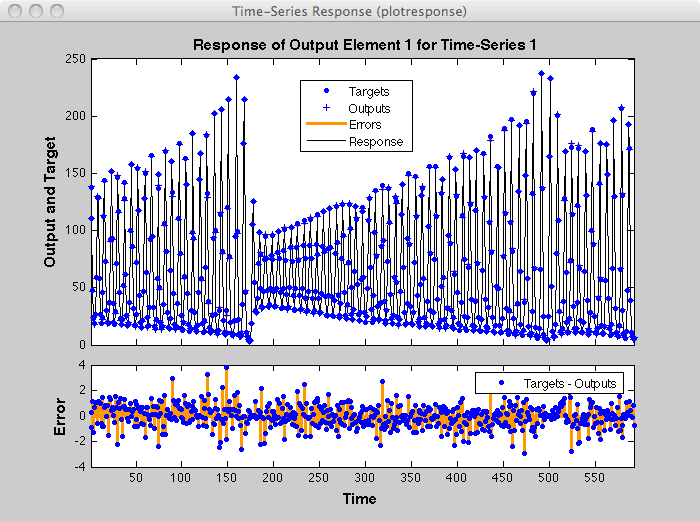
\includegraphics[width=0.8\textwidth]{santafe-matlab.png}
\end{figure}
\end{frame}

\begin{frame}
\frametitle{Neural network: biological}
\begin{figure}[!h]
  \centering
  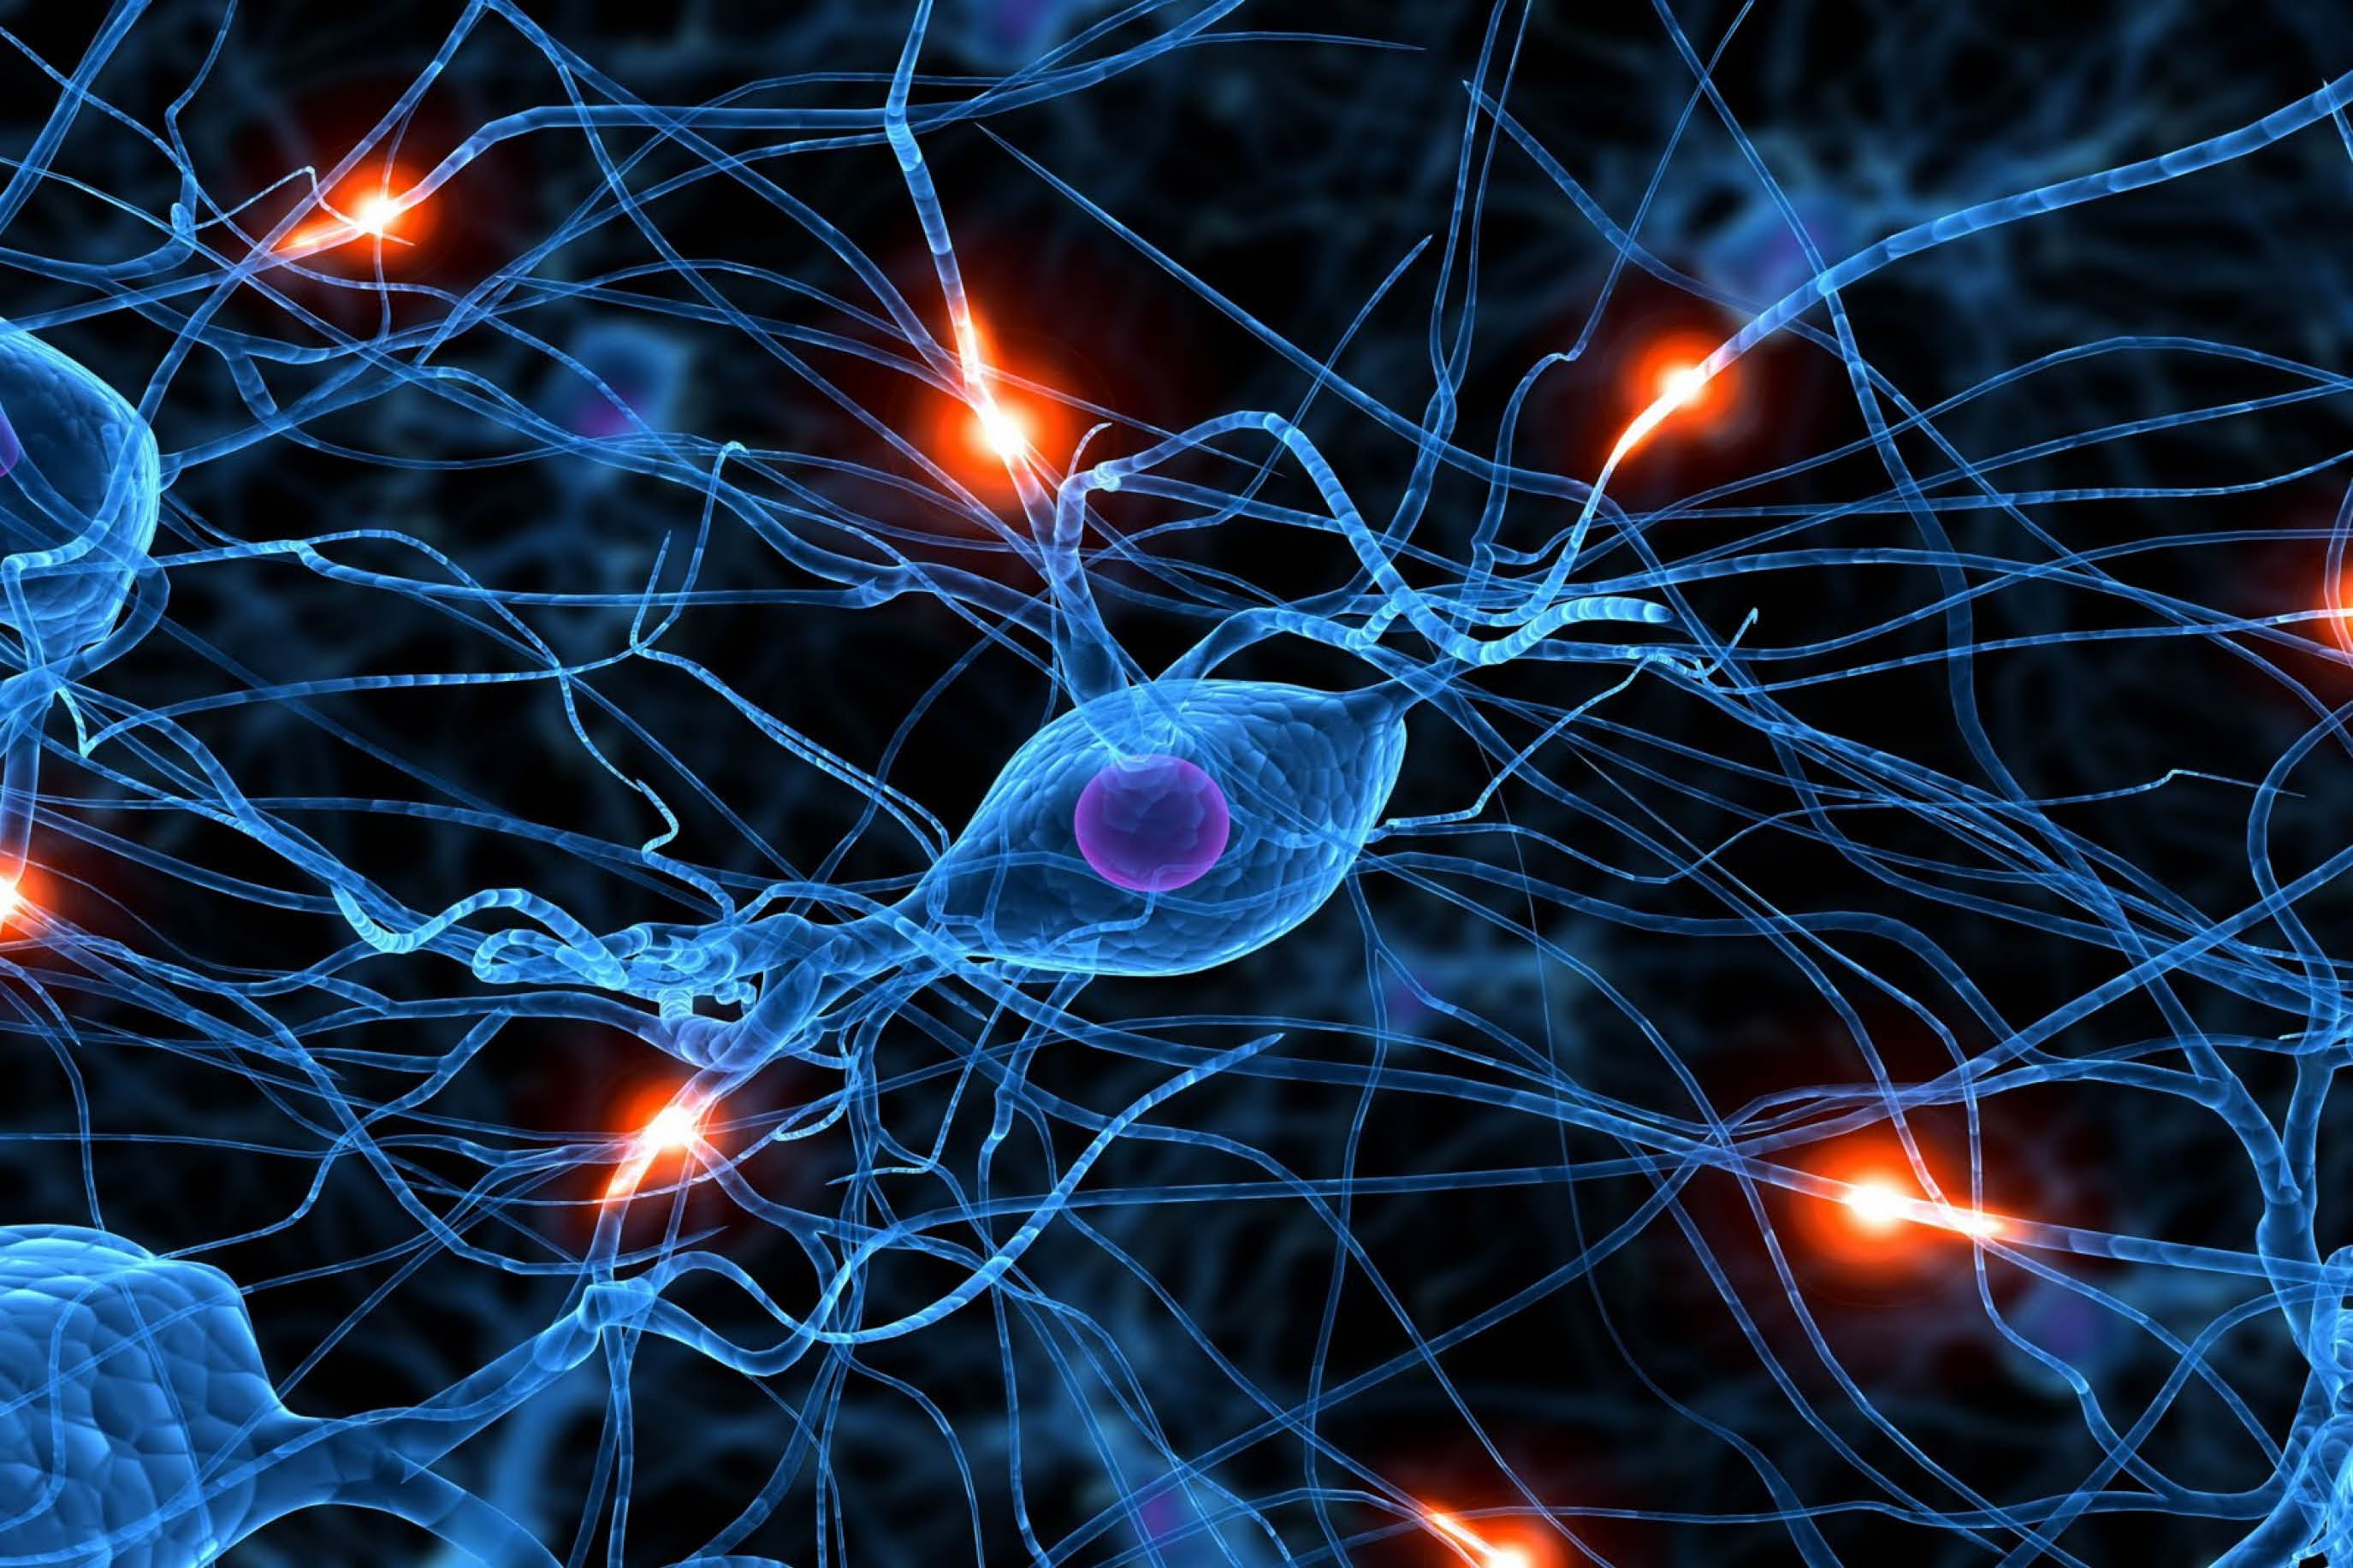
\includegraphics[width=0.9\textwidth]{neural-network-cool.jpg}
\end{figure}
\tiny{Image taken from \url{http://www.extremetech.com/wp-content/uploads/2013/09/340.jpg}}.
\end{frame}

\begin{frame}
\frametitle{Structure of a single neuron}
\begin{figure}[!h]
  \centering
  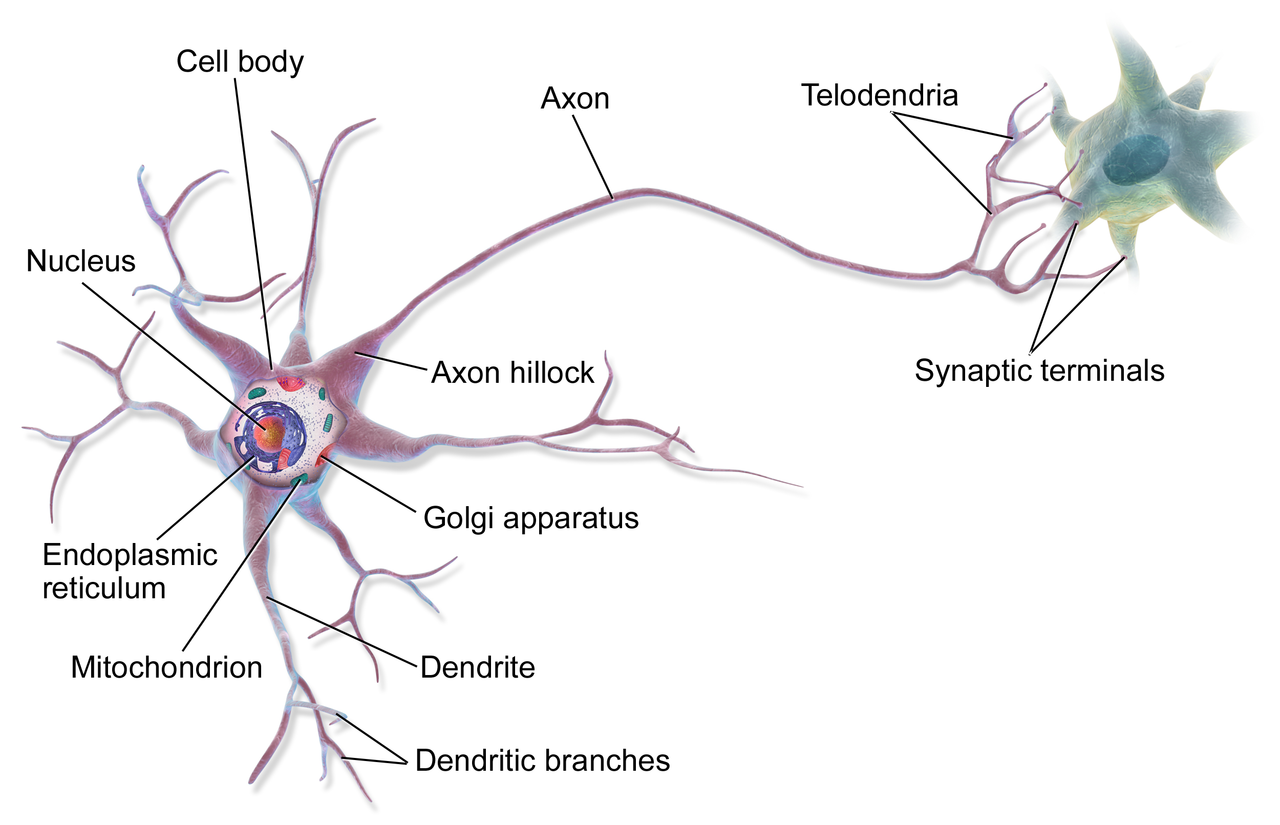
\includegraphics[width=0.9\textwidth]{Blausen_0657_MultipolarNeuron.png}
\end{figure}
\tiny{Image taken from \url{http://en.wikipedia.org/wiki/File:Blausen_0657_MultipolarNeuron.png}}.
\end{frame}


\begin{frame}
\frametitle{Neural network: artificial}
\begin{figure}[!h]
  \centering
  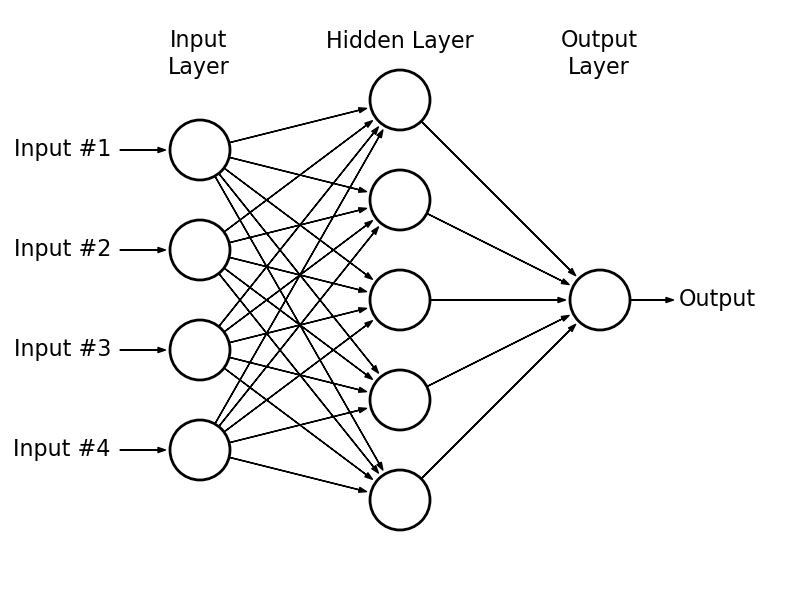
\includegraphics[width=\textwidth]{fig_neural_network_1.png}
\end{figure}
\end{frame}

\begin{frame}
\frametitle{}
\begin{figure}[!h]
  \centering
  
\includegraphics[width=0.7\textwidth]{ask-the-right-questions.jpg}
\end{figure}

\end{frame}

\end{document}
